\documentclass[tikz,border=4pt]{standalone}
\usepackage[T1]{fontenc}
\usepackage{lmodern}
\renewcommand{\familydefault}{\sfdefault}
\usetikzlibrary{shapes.geometric,positioning,arrows.meta,calc,fit,backgrounds,decorations.pathreplacing}
\tikzset{
  node distance=6mm,
  every node/.style={font=\footnotesize,align=center,execute at begin node={\hyphenpenalty=10000\relax}},
  base/.style={draw=gray!60,fill=gray!12,minimum height=7mm,inner sep=2pt},
  term/.style={base,rounded corners=3.5mm,text width=30mm},
  proc/.style={base,text width=32mm},
  err/.style={base,text width=30mm,fill=gray!22},
  io/.style={base,trapezium,trapezium left angle=72,trapezium right angle=108,trapezium stretches=true,text width=28mm},
  dec/.style={base,diamond,aspect=2.4,text width=27mm,inner sep=0pt},
  % predefined process: a call to another procedure
  sub/.style={proc,inner xsep=3mm,path picture={
    \draw[gray!60] ([xshift=1.5mm]path picture bounding box.north west)--([xshift=1.5mm]path picture bounding box.south west)
                   ([xshift=-1.5mm]path picture bounding box.north east)--([xshift=-1.5mm]path picture bounding box.south east);}},
  go/.style={-{Stealth[length=2mm]},draw=gray!55!black},
  lab/.style={font=\scriptsize,fill=white,inner sep=1pt},
  frame/.style={draw=gray!60,dashed,rounded corners=2mm,inner sep=3mm},
  % memory diagrams
  cell/.style={draw=gray!60,fill=gray!12,minimum height=7mm,inner sep=1pt,font=\scriptsize},
  hot/.style={cell,fill=gray!35},
  note/.style={font=\scriptsize,text=gray!30!black},
}

\begin{document}
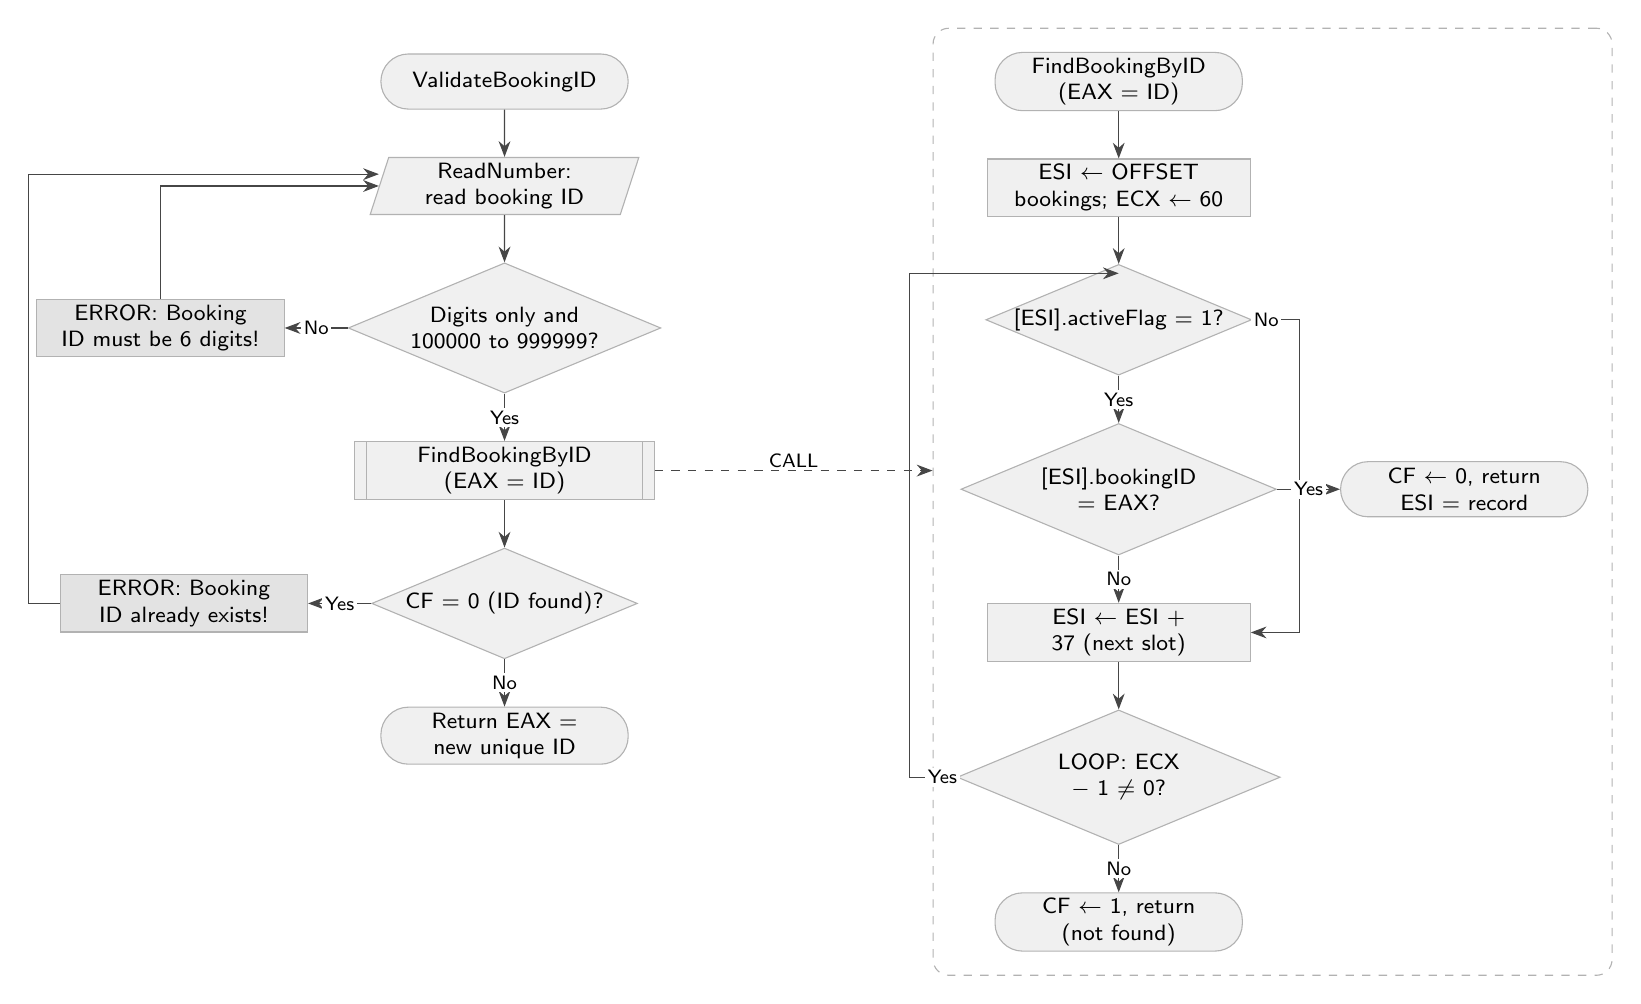
\begin{tikzpicture}
% ValidateBookingID (left column)
\node[term] (s) {ValidateBookingID};
\node[io,below=of s] (r) {ReadNumber: read booking ID};
\node[dec,below=of r] (d1) {Digits only and 100000 to 999999?};
\node[err,left=8mm of d1] (e1) {ERROR: Booking ID must be 6 digits!};
\node[sub,below=of d1] (call) {FindBookingByID (EAX = ID)};
\node[dec,below=of call] (d2) {CF = 0 (ID found)?};
\node[err,left=8mm of d2] (e2) {ERROR: Booking ID already exists!};
\node[term,below=of d2] (ok) {Return EAX = new unique ID};
\draw[go] (s)--(r);
\draw[go] (r)--(d1);
\draw[go] (d1)--node[lab]{No}(e1);
\draw[go] (e1.north)|-(r.west);
\draw[go] (d1)--node[lab]{Yes}(call);
\draw[go] (call)--(d2);
\draw[go] (d2)--node[lab]{Yes}(e2);
\draw[go] (e2.west)--++(-4mm,0)|-([yshift=1.5mm]r.west);
\draw[go] (d2)--node[lab]{No}(ok);
% FindBookingByID (right column)
\node[term] (fs) at ($(s)+(78mm,0)$) {FindBookingByID (EAX = ID)};
\node[proc,below=of fs] (fi) {ESI $\leftarrow$ OFFSET bookings; ECX $\leftarrow$ 60};
\node[dec,below=of fi] (f1) {[ESI].activeFlag = 1?};
\node[dec,below=of f1] (f2) {[ESI].bookingID = EAX?};
\node[term,right=8mm of f2] (found) {CF $\leftarrow$ 0, return ESI = record};
\node[proc,below=of f2] (nx) {ESI $\leftarrow$ ESI + 37 (next slot)};
\node[dec,below=of nx] (f3) {LOOP: ECX $-$ 1 $\neq$ 0?};
\node[term,below=of f3] (nf) {CF $\leftarrow$ 1, return (not found)};
\draw[go] (fs)--(fi);
\draw[go] (fi)--(f1);
\draw[go] (f1)--node[lab]{Yes}(f2);
\draw[go] (f1.east)--node[lab,pos=.3]{No}++(6mm,0)|-(nx.east);
\draw[go] (f2)--node[lab]{Yes}(found);
\draw[go] (f2)--node[lab]{No}(nx);
\draw[go] (nx)--(f3);
\draw[go] (f3)--node[lab]{No}(nf);
\draw[go] (f3.west)--node[lab,pos=.3]{Yes}++(-6mm,0)|-([yshift=-1.2mm]f1.north);
\begin{scope}[on background layer]
\node[frame,fit=(fs)(fi)(f1)(f2)(found)(nx)(f3)(nf)] (box) {};
\end{scope}
\draw[go,dashed] (call.east)--node[lab,above]{CALL}(call.east -| box.west);
\end{tikzpicture}
\end{document}
